\section{Diagrama Entidad Relaci'on}

\begin{figure}[H]
	\begin{center}
		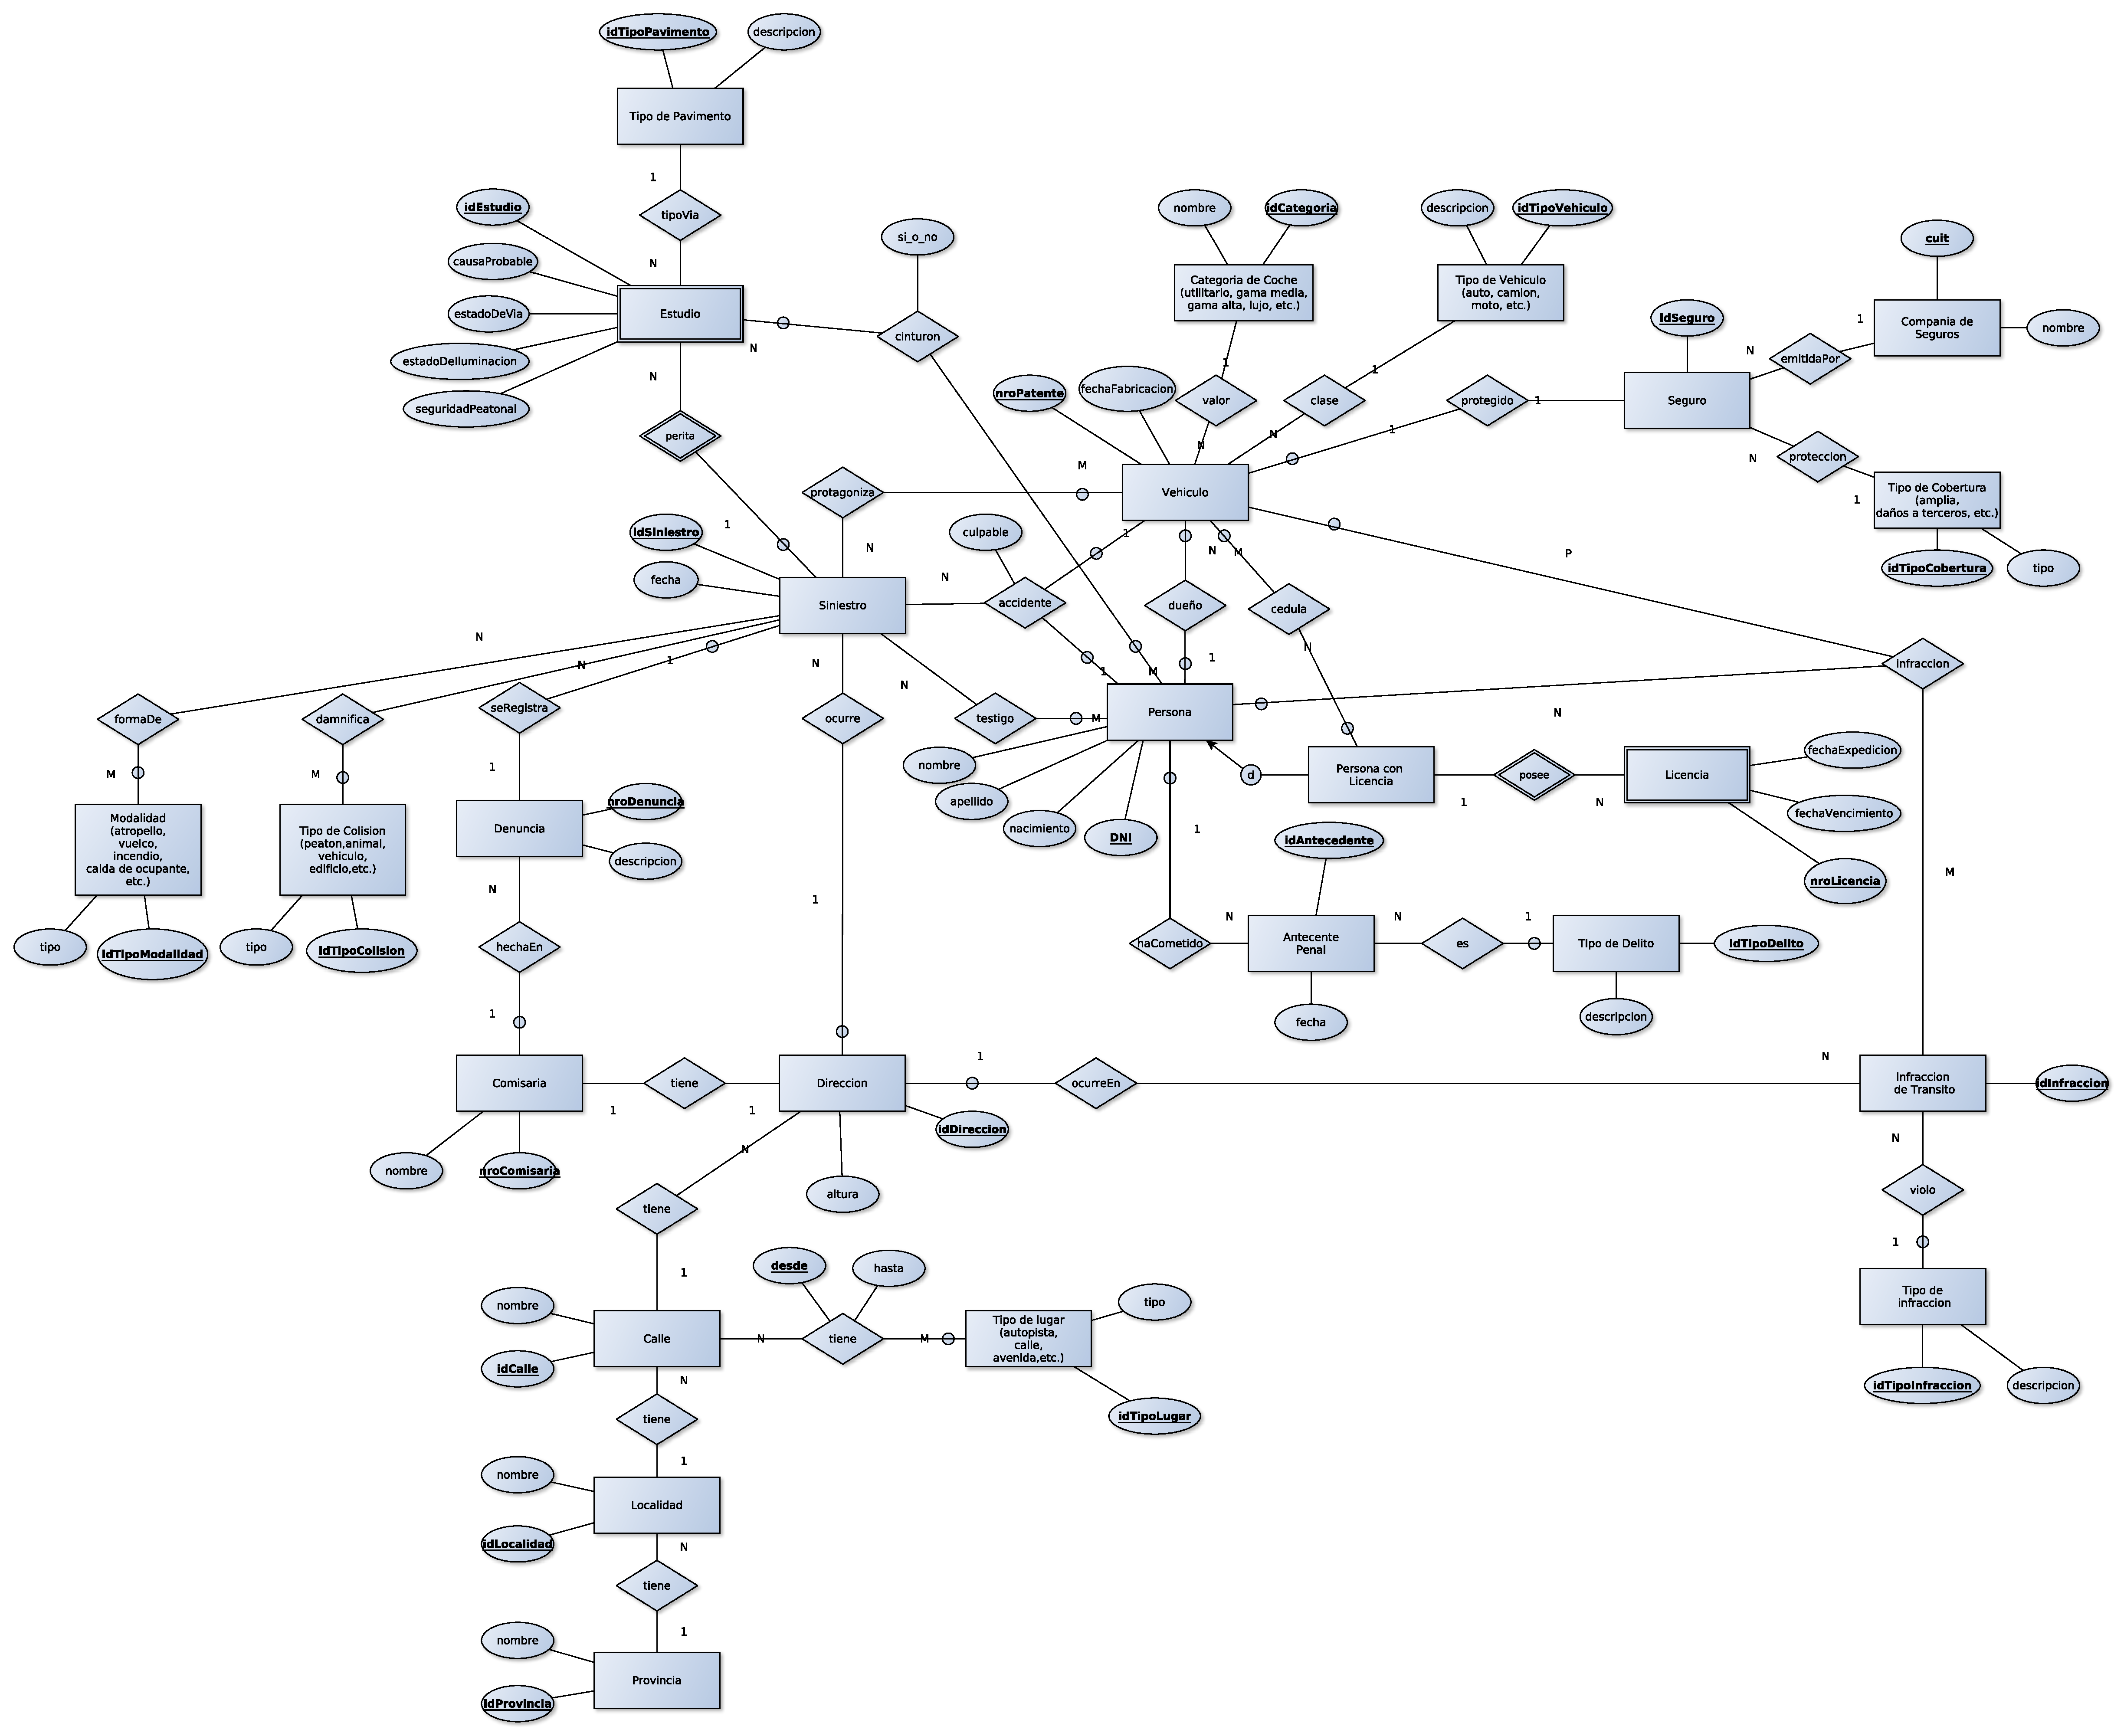
\includegraphics[scale=0.2]{imagenes/DER.pdf}
	\end{center}
\end{figure}

\subsection{Restricciones en lenguaje natural}

\begin{itemize}
\item Los conductores que pertenecen a un estudio, deben ser conductores involucrados en el siniestro de ese estudio.
\item Si un vehiculo aparece relacionado con siniestro sin conductor (en la binaria), entones no aparece en la ternaria. (No tiene sentido que aparezca con y sin conductor). [PENDIENTE: arreglar nombre de las relaciones de siniestro]
\item Las personas que aparecen relacionadas con el estudio en la relacion cinturon, deben ser personas que participaron del siniestro asociado al estudio, conduciendo uno de los vehiculos de ese siniestro.
\end{itemize}
